%\documentclass[11pt]{book}
%
%\setlength{\parindent}{0pt}
%\setlength{\parskip}{8pt}
%
%\usepackage{amsmath}
%\usepackage{amssymb}
%\usepackage{hyperref}
%\usepackage{cleveref}
%
%\renewcommand*{\thefootnote}{\fnsymbol{footnote}}
%
%\setcounter{chapter}{3}
%
%\begin{document}
%
%\section*{A Levelized Comparison of \\ Pulsed and Steady-State Tokamaks}
%
%\let\cleardoublepage\relax \tableofcontents \newpage

\chapter{Completing the Systems Model}

As opposed to previous chapters, this one will focus on the numerics behind the fusion systems model. This will then naturally segue into a discussion of how plots are made and should be interpreted. The remaining chapters will then decouple the dissemination of results and their analytic conclusions.

\section{Describing a Simple Algebra}

Boiled down, the systems model is a simple algebra problem -- given five equations, solve for five unknowns. The goal is then to pick the five equations that best represent modern fusion reactor design. This selection should also be done in such a way that actually reduces the system of equations to a simple univariate root solving equation (i.e. one equation with one unknown). As will be shown in the results, this model does remarkably well: matching year long modeling campaigns in seconds.

The logical place to start in a discussion of this algebra problem is with the three equations fundamental to all reactor-grade tokamaks -- both in steady-state and pulsed operation. These are: the Greenwald density limit, power balance, and current balance. The Greenwald density's importance was hinted early on when it was used to simplify every equation derive thereafter. The two balance equations prove slightly more dubious.

\begin{equation}
	\tag{\ref{eq:greenwald}}
	\overline n = K_n \cdot \frac{I_P}{R_0^2}
\end{equation}

As was shown previously, current balance -- the stability requirement for tokamaks -- was most peculiar. It brought forth the notion of self-consistency for steady-state machines and a highly-coupled multi-root equation for pulsed ones. As such, this equation stands as the one everything else will be substituted into to setup for a univariate root solve.

\begin{equation}
	\tag{\ref{eq:gen_ip}}
	I_P = \frac{ \left( K_{BS} + \sfrac{ G_{IU} }{ G_{IP} } \right) \cdot \overline T }{ 1 - K_{CD} ( \sigma v ) - \sfrac{ G_{ID} }{ G_{IP} } }
\end{equation}

Although slightly buried in \cref{eq:gen_ip}, the right-hand side actually depends on all the quantities (including $I_P$ through the blanket thickness). Through equation,

\begin{equation}
	I_P = f(I_P, \overline T, R_0, B_0)
\end{equation}

The remaining equation common to all reactor-grade tokamaks is power balance -- the relation that separates power plants from toasters. Due to the use of the ELMy H-Mode scaling law for modeling the diffusion coefficient, this had the complicated form of:

\begin{equation}
	\tag{\ref{eq:freidberg}}
	R_0^{ \alpha_R^* } \cdot B_0^{\,\alpha_B} \cdot I_P^{\,\alpha_I^*} = \frac{ G_{PB} }{ K_{PB} }
\end{equation}

Although being rather cumbersome, this equation actually remains relatively simple in that all three quantities on the left-hand side are separable. To close the system, two more equations of this form are needed. These have the following form and will be described next.

\begin{equation}
	\label{eq:rbi}
	R_0^{\, \gamma_R} \cdot B_0^{\, \gamma_B} \cdot I_P^{\, \gamma_I} = G( \overline T )
\end{equation}

\section{Generalizing Previous Equations}

Where the equations defined up to this point in the chapter are shared among all fusion reactors, the remaining two equations needed to close the system must be chosen by the user. These user-supplied equations come in three flavors: limits, derived quantities, and floating variables. By convention, we enforce that at least one limit must be used -- the other constraint can then come from any of the three defined collections.

\begin{table}[hb]
\caption[Main Equation Bank]{Main Equation Bank \\ \small To close the system of equations for potential reactors, different equations can be used to lock down tokamak designs. These include physics and engineering limits (L), as well as ways to set floating (F) or derived (D) variables to constant values.}
\begin{spacing}{1.5}
\begin{tabular}{lccccc}
 Variable & Category & G($\overline T$)  & $\gamma_R$ & $\gamma_B$ & $\gamma_{I}$ \\ \hline
Power Balance & - & $\sfrac{ G_{PB} }{ K_{PB} }$ & $\alpha_R^*$ & $\alpha_B$ & $\alpha_I^*$ \\
Beta ($\beta_N$) & L & $K_{TB} \overline T$ & 1 & 1 & 0 \\
Kink ($q_{95}$) & L & $K_{KF} $ & 1 & 1 & -1 \\
Wall Loading ($P_W$) & L & $K_{WL} ( \sigma v )^{\sfrac{1}{3}} $ & 1 & 0 & -$\sfrac{2}{3}$ \\
Power Cap ($P_E$) & L & $K_{PC} ( \sigma v ) $ & 1 & 0 & -2 \\
Heat Loading ($q_{DV}$) & L & $K_{DV} ( \sigma v )^{\sfrac{1}{3.2}} $ & 1 & 0 & -1 \\
Major Radius ($R_0$) & F & $(R_0)_{const}$ & 1 & 0 & 0 \\
Magnet Strength ($B_0$) & F & $(B_0)_{const}$ & 0 & 1 & 0 \\
Plasma Current ($I_P$) & F & $(I_P)_{const}$ & 0 & 0 & 1 \\
Plasma Temperature ($\overline T$) & F & $\sfrac{ (\overline T)_{const} }{ \, \overline T }$ & 0 & 0 & 0 \\
Electron Density ($\overline n$) & F & $\sfrac{ (\overline n)_{const} }{ K_n }$ & -2 & 0 & 1 \\
Plasma Pressure ($\overline p$) & D & $\sfrac{ (\overline p)_{const} }{ K_n K_{nT} \overline T }$ & -2 & 0 & 1 
\\
Bootstrap Current ($f_{BS}$) & D & $\sfrac{ ( f_{BS} )_{const} }{ K_{BS} \overline T }$ & 0 & 0 & -1 \\
Fusion Power ($P_F$) & D & $\sfrac{ (P_F)_{const} }{ K_F K_n ^ 2 ( \sigma v ) }$ & -1 & 0 & 2 \\
Magnetic Energy ($W_M$) & D & $\sfrac{ (W_M)_{const} }{ K_{WM} }$ & 3 & 2 & 0 \\
Cost per Watt ($C_W$) & D & $ (C_W)_{const} \cdot \left( \sfrac{ K_F K_n ^ 2 ( \sigma v ) }{ K_{WM} } \right)$ & 4 & 2 & -2 \\
\end{tabular}
\end{spacing}
\label{table:eq}
\end{table}

\subsection{Rehashing the Limits}

The limits category is simply a rebranding of the secondary constraints given previously. These were the physics derived limits from MHD theory -- i.e. the beta limit ($\beta_N$) and the kink safety factor ($q_{95}$) -- which for clarity, set maximums on the allowed plasma pressure and velocity, respectively. Additionally, there were engineering limits from: wall loading, heat loading, and maximum power capacity. For this paper, wall loading from neutrons ($P_W$) is assumed to be important, whereas the other two are not allowed to explicitly guide designs.

Combined all these limits, as well as the yet to be defined float and derived equations, are given in \cref{table:eq}. These share a remarkably similar form to power balance when put into a generalized, separable state. This hints at why the major radius ($R_0$), the toroidal field strength ($B_0$), and the plasma current ($I_P$) can easily be separated and substituted out of the current balance equation.

Before moving on, it proves useful to explain the two limits not used to explicitly guide reactor design -- divertor heat loading and a maximum power capacity. The simpler of the two to reason is the heat loading limit. Although removing the gigawatts of heat is extremely difficult, it remains an unsolved problem worthy of its own research machine, but currently neglected financially. As such, it is only kept to provide a human-interpreted  measure of difficulty. The power cap, on the other hand, is just handled informally. If a reactor surpasses it (i.e. $ P_E > 4000 MW $), it is considered invalid.

While the maximum power cap informally sets a maximum major radius for a machine, there also exists an implicit minimum major radius. This minimum occurs due to the hole-size constraint -- i.e. at some point there is no longer enough room on the inside of the machine to store the central solenoid, blanket, and TF coils.

At this point, we can now explain how various quantities in the systems model can be set to user-given constant values. This basically allows users to treat one floating variable as a fixed one (e.g. the temperature).

\subsection{Minimizing Derived Quantities} 

Whereas the limits from the previous section represented constraints with real physics and engineering repercussions, the derived quantities here are just used to find when reactors reach certain user-supplied values. Most notable are the capital cost (through the magnetic energy -- $W_M$) and the cost-per-watt ($C_W$). The model also, however, allows easily setting values for the bootstrap fraction, plasma pressure, and fusion power. As mentioned previously, they are given in \cref{table:eq} through a generalized representation of the form:

\begin{equation}
	\tag{\ref{eq:rbi}}
	R_0^{\, \gamma_R} \cdot B_0^{\, \gamma_B} \cdot I_P^{\, \gamma_I} = G( \overline T )
\end{equation}

What this collection of variables is really useful for, though, is finding minimum cost reactors -- both in a capital context as well as a cost-per-watt one. Without boring the reader, this is done in a three stage process. First, some valid reactor is found: it does not matter if it is good, just valid. This of course can be found by systematically throwing darts at a dart board. 

\begin{figure}[h]
\centering
\begin{adjustbox}{width=0.8\textwidth}
	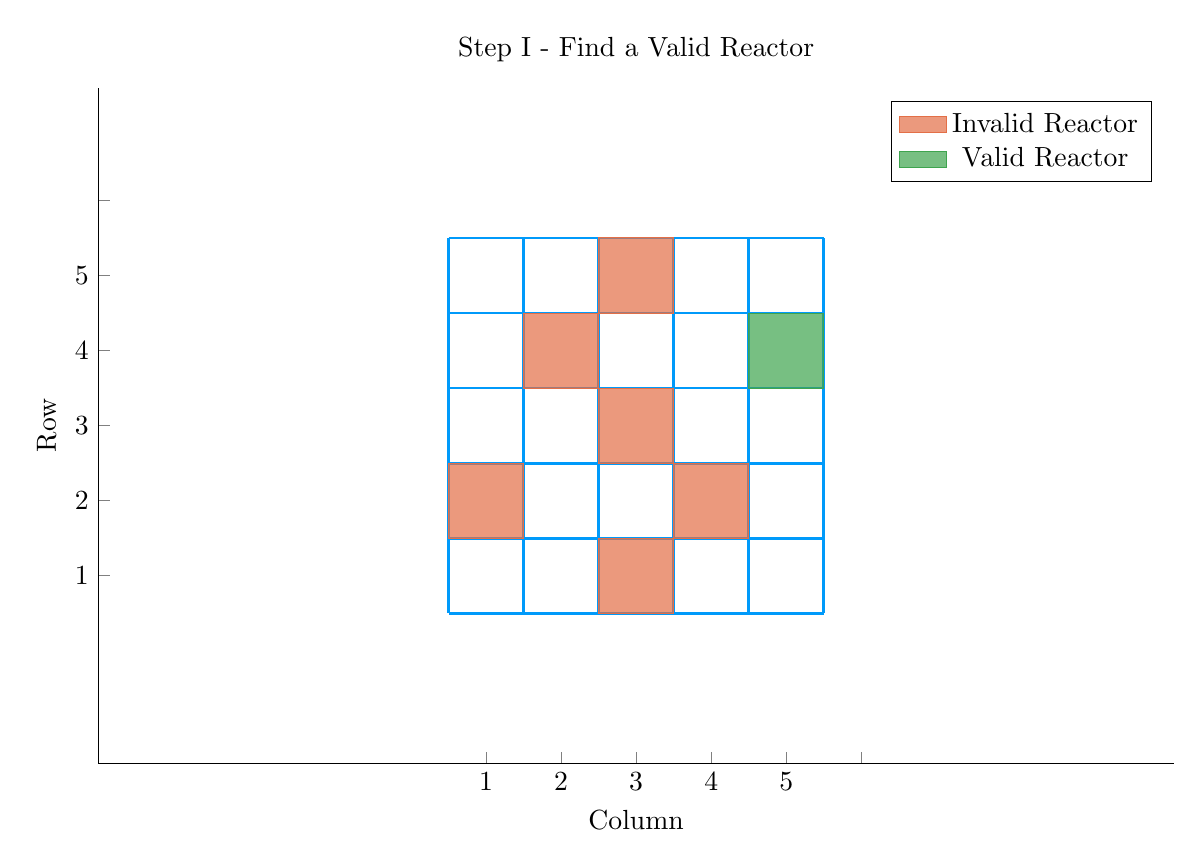
\begin{tikzpicture}[]
\begin{axis}[height = {101.6mm}, axis equal = {true}, ylabel = {Row}, title = {Step I - Find a Valid Reactor}, xmin = {0.0}, xmax = {5.0}, ymax = {7}, xlabel = {Column}, {unbounded coords=jump, xticklabel style={rotate = 0}, xmajorgrids = false, xtick = {0.5,1.5,2.5,3.5,4.5,5.5}, xticklabels = {1,2,3,4,5}, xtick align = inside, axis lines* = left, yticklabel style={rotate = 0}, ymajorgrids = false, ytick = {0.5,1.5,2.5,3.5,4.5,5.5}, yticklabels = {1,2,3,4,5}, ytick align = inside, axis lines* = left,     xshift = 0.0mm,
    yshift = 0.0mm,
    axis background/.style={fill={rgb,1:red,1.00000000;green,1.00000000;blue,1.00000000}}
}, ymin = {-2}, width = {152.4mm}]\addplot+ [color = {rgb,1:red,0.00000000;green,0.60560316;blue,0.97868012},
draw opacity=1.0,
line width=1,
solid,mark = none,
mark size = 2.0,
mark options = {
    color = {rgb,1:red,0.00000000;green,0.00000000;blue,0.00000000}, draw opacity = 1.0,
    fill = {rgb,1:red,0.00000000;green,0.60560316;blue,0.97868012}, fill opacity = 1.0,
    line width = 1,
    rotate = 0,
    solid
},forget plot]coordinates {
(0, 0)
(0, 5)
};
\addplot+ [color = {rgb,1:red,0.00000000;green,0.60560316;blue,0.97868012},
draw opacity=1.0,
line width=1,
solid,mark = none,
mark size = 2.0,
mark options = {
    color = {rgb,1:red,0.00000000;green,0.00000000;blue,0.00000000}, draw opacity = 1.0,
    fill = {rgb,1:red,0.00000000;green,0.60560316;blue,0.97868012}, fill opacity = 1.0,
    line width = 1,
    rotate = 0,
    solid
},forget plot]coordinates {
(0, 0)
(5, 0)
};
\addplot+ [color = {rgb,1:red,0.00000000;green,0.60560316;blue,0.97868012},
draw opacity=1.0,
line width=1,
solid,mark = none,
mark size = 2.0,
mark options = {
    color = {rgb,1:red,0.00000000;green,0.00000000;blue,0.00000000}, draw opacity = 1.0,
    fill = {rgb,1:red,0.00000000;green,0.60560316;blue,0.97868012}, fill opacity = 1.0,
    line width = 1,
    rotate = 0,
    solid
},forget plot]coordinates {
(1, 0)
(1, 5)
};
\addplot+ [color = {rgb,1:red,0.00000000;green,0.60560316;blue,0.97868012},
draw opacity=1.0,
line width=1,
solid,mark = none,
mark size = 2.0,
mark options = {
    color = {rgb,1:red,0.00000000;green,0.00000000;blue,0.00000000}, draw opacity = 1.0,
    fill = {rgb,1:red,0.00000000;green,0.60560316;blue,0.97868012}, fill opacity = 1.0,
    line width = 1,
    rotate = 0,
    solid
},forget plot]coordinates {
(0, 1)
(5, 1)
};
\addplot+ [color = {rgb,1:red,0.00000000;green,0.60560316;blue,0.97868012},
draw opacity=1.0,
line width=1,
solid,mark = none,
mark size = 2.0,
mark options = {
    color = {rgb,1:red,0.00000000;green,0.00000000;blue,0.00000000}, draw opacity = 1.0,
    fill = {rgb,1:red,0.00000000;green,0.60560316;blue,0.97868012}, fill opacity = 1.0,
    line width = 1,
    rotate = 0,
    solid
},forget plot]coordinates {
(2, 0)
(2, 5)
};
\addplot+ [color = {rgb,1:red,0.00000000;green,0.60560316;blue,0.97868012},
draw opacity=1.0,
line width=1,
solid,mark = none,
mark size = 2.0,
mark options = {
    color = {rgb,1:red,0.00000000;green,0.00000000;blue,0.00000000}, draw opacity = 1.0,
    fill = {rgb,1:red,0.00000000;green,0.60560316;blue,0.97868012}, fill opacity = 1.0,
    line width = 1,
    rotate = 0,
    solid
},forget plot]coordinates {
(0, 2)
(5, 2)
};
\addplot+ [color = {rgb,1:red,0.00000000;green,0.60560316;blue,0.97868012},
draw opacity=1.0,
line width=1,
solid,mark = none,
mark size = 2.0,
mark options = {
    color = {rgb,1:red,0.00000000;green,0.00000000;blue,0.00000000}, draw opacity = 1.0,
    fill = {rgb,1:red,0.00000000;green,0.60560316;blue,0.97868012}, fill opacity = 1.0,
    line width = 1,
    rotate = 0,
    solid
},forget plot]coordinates {
(3, 0)
(3, 5)
};
\addplot+ [color = {rgb,1:red,0.00000000;green,0.60560316;blue,0.97868012},
draw opacity=1.0,
line width=1,
solid,mark = none,
mark size = 2.0,
mark options = {
    color = {rgb,1:red,0.00000000;green,0.00000000;blue,0.00000000}, draw opacity = 1.0,
    fill = {rgb,1:red,0.00000000;green,0.60560316;blue,0.97868012}, fill opacity = 1.0,
    line width = 1,
    rotate = 0,
    solid
},forget plot]coordinates {
(0, 3)
(5, 3)
};
\addplot+ [color = {rgb,1:red,0.00000000;green,0.60560316;blue,0.97868012},
draw opacity=1.0,
line width=1,
solid,mark = none,
mark size = 2.0,
mark options = {
    color = {rgb,1:red,0.00000000;green,0.00000000;blue,0.00000000}, draw opacity = 1.0,
    fill = {rgb,1:red,0.00000000;green,0.60560316;blue,0.97868012}, fill opacity = 1.0,
    line width = 1,
    rotate = 0,
    solid
},forget plot]coordinates {
(4, 0)
(4, 5)
};
\addplot+ [color = {rgb,1:red,0.00000000;green,0.60560316;blue,0.97868012},
draw opacity=1.0,
line width=1,
solid,mark = none,
mark size = 2.0,
mark options = {
    color = {rgb,1:red,0.00000000;green,0.00000000;blue,0.00000000}, draw opacity = 1.0,
    fill = {rgb,1:red,0.00000000;green,0.60560316;blue,0.97868012}, fill opacity = 1.0,
    line width = 1,
    rotate = 0,
    solid
},forget plot]coordinates {
(0, 4)
(5, 4)
};
\addplot+ [color = {rgb,1:red,0.00000000;green,0.60560316;blue,0.97868012},
draw opacity=1.0,
line width=1,
solid,mark = none,
mark size = 2.0,
mark options = {
    color = {rgb,1:red,0.00000000;green,0.00000000;blue,0.00000000}, draw opacity = 1.0,
    fill = {rgb,1:red,0.00000000;green,0.60560316;blue,0.97868012}, fill opacity = 1.0,
    line width = 1,
    rotate = 0,
    solid
},forget plot]coordinates {
(5, 0)
(5, 5)
};
\addplot+ [color = {rgb,1:red,0.00000000;green,0.60560316;blue,0.97868012},
draw opacity=1.0,
line width=1,
solid,mark = none,
mark size = 2.0,
mark options = {
    color = {rgb,1:red,0.00000000;green,0.00000000;blue,0.00000000}, draw opacity = 1.0,
    fill = {rgb,1:red,0.00000000;green,0.60560316;blue,0.97868012}, fill opacity = 1.0,
    line width = 1,
    rotate = 0,
    solid
},forget plot]coordinates {
(0, 5)
(5, 5)
};
\addplot+ [color = {rgb,1:red,0.88887350;green,0.43564919;blue,0.27812294},
draw opacity=1.0,
line width=0,
solid,mark = none,
mark size = 2.0,
mark options = {
    color = {rgb,1:red,0.00000000;green,0.00000000;blue,0.00000000}, draw opacity = 1.0,
    fill = {rgb,1:red,0.88887350;green,0.43564919;blue,0.27812294}, fill opacity = 1.0,
    line width = 1,
    rotate = 0,
    solid
},fill = {rgb,1:red,0.88887350;green,0.43564919;blue,0.27812294}, fill opacity=0.7,area legend]coordinates {
(2, 2)
(2, 3)
(3, 3)
(3, 2)
(2, 2)
};
\addlegendentry{Invalid Reactor}
\addplot+ [color = {rgb,1:red,0.88887350;green,0.43564919;blue,0.27812294},
draw opacity=1.0,
line width=0,
solid,mark = none,
mark size = 2.0,
mark options = {
    color = {rgb,1:red,0.00000000;green,0.00000000;blue,0.00000000}, draw opacity = 1.0,
    fill = {rgb,1:red,0.88887350;green,0.43564919;blue,0.27812294}, fill opacity = 1.0,
    line width = 1,
    rotate = 0,
    solid
},fill = {rgb,1:red,0.88887350;green,0.43564919;blue,0.27812294}, fill opacity=0.7,forget plot]coordinates {
(1, 3)
(1, 4)
(2, 4)
(2, 3)
(1, 3)
};
\addplot+ [color = {rgb,1:red,0.88887350;green,0.43564919;blue,0.27812294},
draw opacity=1.0,
line width=0,
solid,mark = none,
mark size = 2.0,
mark options = {
    color = {rgb,1:red,0.00000000;green,0.00000000;blue,0.00000000}, draw opacity = 1.0,
    fill = {rgb,1:red,0.88887350;green,0.43564919;blue,0.27812294}, fill opacity = 1.0,
    line width = 1,
    rotate = 0,
    solid
},fill = {rgb,1:red,0.88887350;green,0.43564919;blue,0.27812294}, fill opacity=0.7,forget plot]coordinates {
(3, 1)
(3, 2)
(4, 2)
(4, 1)
(3, 1)
};
\addplot+ [color = {rgb,1:red,0.88887350;green,0.43564919;blue,0.27812294},
draw opacity=1.0,
line width=0,
solid,mark = none,
mark size = 2.0,
mark options = {
    color = {rgb,1:red,0.00000000;green,0.00000000;blue,0.00000000}, draw opacity = 1.0,
    fill = {rgb,1:red,0.88887350;green,0.43564919;blue,0.27812294}, fill opacity = 1.0,
    line width = 1,
    rotate = 0,
    solid
},fill = {rgb,1:red,0.88887350;green,0.43564919;blue,0.27812294}, fill opacity=0.7,forget plot]coordinates {
(2, 4)
(2, 5)
(3, 5)
(3, 4)
(2, 4)
};
\addplot+ [color = {rgb,1:red,0.88887350;green,0.43564919;blue,0.27812294},
draw opacity=1.0,
line width=0,
solid,mark = none,
mark size = 2.0,
mark options = {
    color = {rgb,1:red,0.00000000;green,0.00000000;blue,0.00000000}, draw opacity = 1.0,
    fill = {rgb,1:red,0.88887350;green,0.43564919;blue,0.27812294}, fill opacity = 1.0,
    line width = 1,
    rotate = 0,
    solid
},fill = {rgb,1:red,0.88887350;green,0.43564919;blue,0.27812294}, fill opacity=0.7,forget plot]coordinates {
(0, 1)
(0, 2)
(1, 2)
(1, 1)
(0, 1)
};
\addplot+ [color = {rgb,1:red,0.88887350;green,0.43564919;blue,0.27812294},
draw opacity=1.0,
line width=0,
solid,mark = none,
mark size = 2.0,
mark options = {
    color = {rgb,1:red,0.00000000;green,0.00000000;blue,0.00000000}, draw opacity = 1.0,
    fill = {rgb,1:red,0.88887350;green,0.43564919;blue,0.27812294}, fill opacity = 1.0,
    line width = 1,
    rotate = 0,
    solid
},fill = {rgb,1:red,0.88887350;green,0.43564919;blue,0.27812294}, fill opacity=0.7,forget plot]coordinates {
(2, 0)
(2, 1)
(3, 1)
(3, 0)
(2, 0)
};
\addplot+ [color = {rgb,1:red,0.24222430;green,0.64327509;blue,0.30444865},
draw opacity=1.0,
line width=0,
solid,mark = none,
mark size = 2.0,
mark options = {
    color = {rgb,1:red,0.00000000;green,0.00000000;blue,0.00000000}, draw opacity = 1.0,
    fill = {rgb,1:red,0.24222430;green,0.64327509;blue,0.30444865}, fill opacity = 1.0,
    line width = 1,
    rotate = 0,
    solid
},fill = {rgb,1:red,0.24222430;green,0.64327509;blue,0.30444865}, fill opacity=0.7,area legend]coordinates {
(4, 3)
(4, 4)
(5, 4)
(5, 3)
(4, 3)
};
\addlegendentry{Valid Reactor}
\end{axis}

\end{tikzpicture}

\end{adjustbox}
\caption{Minimize Cost Step I -- Find Valid Reactor}
\label{fig:step_one}
\end{figure}

After a valid reactor is found, its cost is recorded leading to a drill-down stage. In this step, the cost is continuously halved until a valid one cannot be found. Once this invalid reactor is reached, it sets a bound on the minimum cost reactor. As such, the final stage is a simple bisection step where the minimum cost is honed down to some acceptable margin of error -- see \cref{fig:minimize}.

\begin{figure*}
    \centering
    \begin{subfigure}[t]{0.8\textwidth}
        \centering
		\begin{adjustbox}{width=\textwidth}
			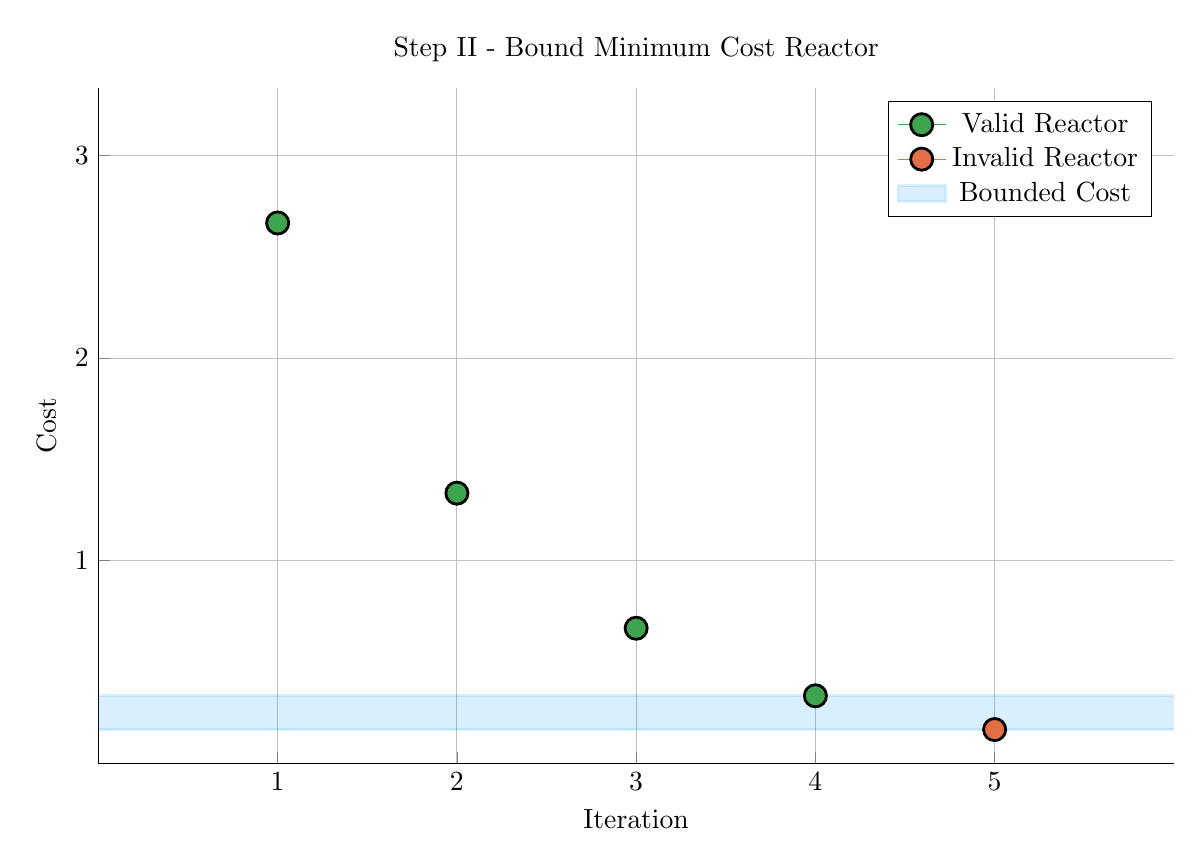
\begin{tikzpicture}[]
\begin{axis}[height = {101.6mm}, ylabel = {Cost}, title = {Step II - Bound Minimum Cost Reactor}, xmin = {0}, xmax = {6}, ymax = {40}, xlabel = {Iteration}, {unbounded coords=jump, xticklabel style={rotate = 0}, xmajorgrids = true, xtick = {1.0,2.0,3.0,4.0,5.0}, xticklabels = {1,2,3,4,5}, xtick align = inside, axis lines* = left, yticklabel style={rotate = 0}, ymajorgrids = true, ytick = {12,24,36}, yticklabels = {1,2,3}, ytick align = inside, axis lines* = left,     xshift = 0.0mm,
    yshift = 0.0mm,
    axis background/.style={fill={rgb,1:red,1.00000000;green,1.00000000;blue,1.00000000}}
}, ymin = {0}, width = {152.4mm}]\addplot+[draw=none, color = {rgb,1:red,0.24222430;green,0.64327509;blue,0.30444865},
draw opacity=1.0,
line width=0,
solid,mark = *,
mark size = 4.0,
mark options = {
    color = {rgb,1:red,0.00000000;green,0.00000000;blue,0.00000000}, draw opacity = 1.0,
    fill = {rgb,1:red,0.24222430;green,0.64327509;blue,0.30444865}, fill opacity = 1.0,
    line width = 1,
    rotate = 0,
    solid
}] coordinates {
(1.0, 32.0)
};
\addlegendentry{Valid Reactor}
\addplot+[draw=none, color = {rgb,1:red,0.24222430;green,0.64327509;blue,0.30444865},
draw opacity=1.0,
line width=0,
solid,mark = *,
mark size = 4.0,
mark options = {
    color = {rgb,1:red,0.00000000;green,0.00000000;blue,0.00000000}, draw opacity = 1.0,
    fill = {rgb,1:red,0.24222430;green,0.64327509;blue,0.30444865}, fill opacity = 1.0,
    line width = 1,
    rotate = 0,
    solid
},forget plot] coordinates {
(2.0, 16.0)
};
\addplot+[draw=none, color = {rgb,1:red,0.24222430;green,0.64327509;blue,0.30444865},
draw opacity=1.0,
line width=0,
solid,mark = *,
mark size = 4.0,
mark options = {
    color = {rgb,1:red,0.00000000;green,0.00000000;blue,0.00000000}, draw opacity = 1.0,
    fill = {rgb,1:red,0.24222430;green,0.64327509;blue,0.30444865}, fill opacity = 1.0,
    line width = 1,
    rotate = 0,
    solid
},forget plot] coordinates {
(3.0, 8.0)
};
\addplot+[draw=none, color = {rgb,1:red,0.24222430;green,0.64327509;blue,0.30444865},
draw opacity=1.0,
line width=0,
solid,mark = *,
mark size = 4.0,
mark options = {
    color = {rgb,1:red,0.00000000;green,0.00000000;blue,0.00000000}, draw opacity = 1.0,
    fill = {rgb,1:red,0.24222430;green,0.64327509;blue,0.30444865}, fill opacity = 1.0,
    line width = 1,
    rotate = 0,
    solid
},forget plot] coordinates {
(4.0, 4.0)
};
\addplot+[draw=none, color = {rgb,1:red,0.88887350;green,0.43564919;blue,0.27812294},
draw opacity=1.0,
line width=0,
solid,mark = *,
mark size = 4.0,
mark options = {
    color = {rgb,1:red,0.00000000;green,0.00000000;blue,0.00000000}, draw opacity = 1.0,
    fill = {rgb,1:red,0.88887350;green,0.43564919;blue,0.27812294}, fill opacity = 1.0,
    line width = 1,
    rotate = 0,
    solid
}] coordinates {
(5.0, 2.0)
};
\addlegendentry{Invalid Reactor}
\addplot+ [color = {rgb,1:red,0.00000000;green,0.60560316;blue,0.97868012},
draw opacity=0.15,
line width=1,
solid,mark = none,
mark size = 2.0,
mark options = {
    color = {rgb,1:red,0.00000000;green,0.00000000;blue,0.00000000}, draw opacity = 0.15,
    fill = {rgb,1:red,0.00000000;green,0.60560316;blue,0.97868012}, fill opacity = 0.15,
    line width = 1,
    rotate = 0,
    solid
},fill = {rgb,1:red,0.00000000;green,0.60560316;blue,0.97868012}, fill opacity=0.15,area legend]coordinates {
(-1.0, 4.0)
(-1.0, 2.0)
(7.0, 2.0)
(7.0, 4.0)
(-1.0, 4.0)
};
\addlegendentry{Bounded Cost}
\end{axis}

\end{tikzpicture}

		\end{adjustbox}
        \caption{ Minimize Step II }
    \end{subfigure} 
    \par \bigskip \par \bigskip 
    \begin{subfigure}[t]{0.8\textwidth}
        \centering
		\begin{adjustbox}{width=\textwidth}
			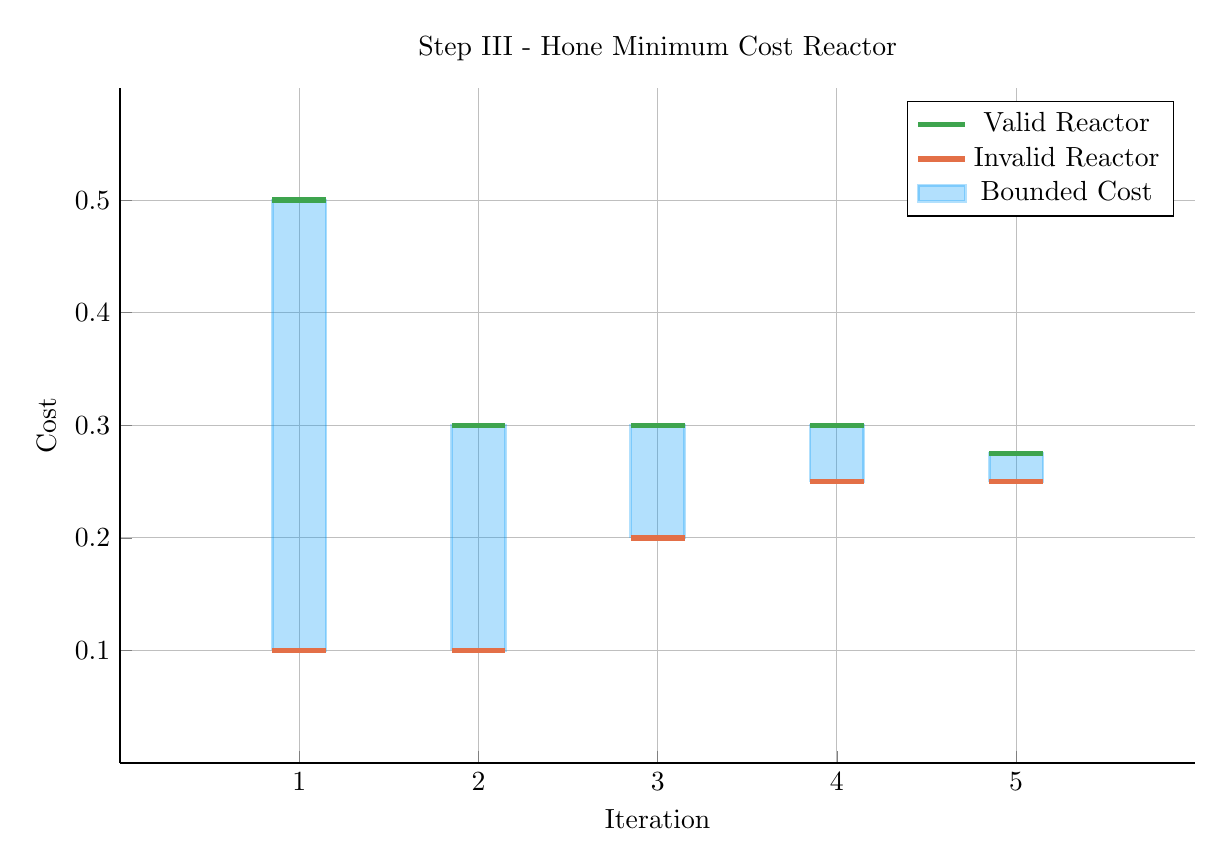
\begin{tikzpicture}[]
\begin{axis}[height = {101.6mm}, ylabel = {Cost}, title = {Step III - Hone Minimum Cost Reactor}, xmin = {0}, xmax = {6}, ymax = {0.6}, xlabel = {Iteration}, {unbounded coords=jump, xticklabel style={rotate = 0}, xmajorgrids = true, xtick = {1.0,2.0,3.0,4.0,5.0}, xticklabels = {1,2,3,4,5}, xtick align = inside, axis lines* = left, yticklabel style={rotate = 0}, ymajorgrids = true, ytick = {0.1,0.2,0.3,0.4,0.5}, yticklabels = {0.1,0.2,0.3,0.4,0.5}, ytick align = inside, axis lines* = left,     xshift = 0.0mm,
    yshift = 0.0mm,
    axis background/.style={fill={rgb,1:red,1.00000000;green,1.00000000;blue,1.00000000}}
}, ymin = {0}, width = {152.4mm}]\addplot+ [color = {rgb,1:red,0.00000000;green,0.60560316;blue,0.97868012},
draw opacity=0.3,
line width=1,
solid,mark = none,
mark size = 2.0,
mark options = {
    color = {rgb,1:red,0.00000000;green,0.00000000;blue,0.00000000}, draw opacity = 0.3,
    fill = {rgb,1:red,0.00000000;green,0.60560316;blue,0.97868012}, fill opacity = 0.3,
    line width = 1,
    rotate = 0,
    solid
},fill = {rgb,1:red,0.00000000;green,0.60560316;blue,0.97868012}, fill opacity=0.3,forget plot]coordinates {
(0.85, 0.1)
(0.85, 0.5)
(1.15, 0.5)
(1.15, 0.1)
(0.85, 0.1)
};
\addplot+ [color = {rgb,1:red,0.24222430;green,0.64327509;blue,0.30444865},
draw opacity=1.0,
line width=2,
solid,mark = none,
mark size = 2.0,
mark options = {
    color = {rgb,1:red,0.00000000;green,0.00000000;blue,0.00000000}, draw opacity = 1.0,
    fill = {rgb,1:red,0.24222430;green,0.64327509;blue,0.30444865}, fill opacity = 1.0,
    line width = 1,
    rotate = 0,
    solid
}]coordinates {
(0.85, 0.5)
(1.15, 0.5)
};
\addlegendentry{Valid Reactor}
\addplot+ [color = {rgb,1:red,0.88887350;green,0.43564919;blue,0.27812294},
draw opacity=1.0,
line width=2,
solid,mark = none,
mark size = 2.0,
mark options = {
    color = {rgb,1:red,0.00000000;green,0.00000000;blue,0.00000000}, draw opacity = 1.0,
    fill = {rgb,1:red,0.88887350;green,0.43564919;blue,0.27812294}, fill opacity = 1.0,
    line width = 1,
    rotate = 0,
    solid
}]coordinates {
(0.85, 0.1)
(1.15, 0.1)
};
\addlegendentry{Invalid Reactor}
\addplot+ [color = {rgb,1:red,0.00000000;green,0.60560316;blue,0.97868012},
draw opacity=0.3,
line width=1,
solid,mark = none,
mark size = 2.0,
mark options = {
    color = {rgb,1:red,0.00000000;green,0.00000000;blue,0.00000000}, draw opacity = 0.3,
    fill = {rgb,1:red,0.00000000;green,0.60560316;blue,0.97868012}, fill opacity = 0.3,
    line width = 1,
    rotate = 0,
    solid
},fill = {rgb,1:red,0.00000000;green,0.60560316;blue,0.97868012}, fill opacity=0.3,area legend]coordinates {
(1.85, 0.1)
(1.85, 0.3)
(2.15, 0.3)
(2.15, 0.1)
(1.85, 0.1)
};
\addlegendentry{Bounded Cost}
\addplot+ [color = {rgb,1:red,0.88887350;green,0.43564919;blue,0.27812294},
draw opacity=1.0,
line width=2,
solid,mark = none,
mark size = 2.0,
mark options = {
    color = {rgb,1:red,0.00000000;green,0.00000000;blue,0.00000000}, draw opacity = 1.0,
    fill = {rgb,1:red,0.88887350;green,0.43564919;blue,0.27812294}, fill opacity = 1.0,
    line width = 1,
    rotate = 0,
    solid
},forget plot]coordinates {
(1.85, 0.1)
(2.15, 0.1)
};
\addplot+ [color = {rgb,1:red,0.24222430;green,0.64327509;blue,0.30444865},
draw opacity=1.0,
line width=2,
solid,mark = none,
mark size = 2.0,
mark options = {
    color = {rgb,1:red,0.00000000;green,0.00000000;blue,0.00000000}, draw opacity = 1.0,
    fill = {rgb,1:red,0.24222430;green,0.64327509;blue,0.30444865}, fill opacity = 1.0,
    line width = 1,
    rotate = 0,
    solid
},forget plot]coordinates {
(1.85, 0.3)
(2.15, 0.3)
};
\addplot+ [color = {rgb,1:red,0.00000000;green,0.60560316;blue,0.97868012},
draw opacity=0.3,
line width=1,
solid,mark = none,
mark size = 2.0,
mark options = {
    color = {rgb,1:red,0.00000000;green,0.00000000;blue,0.00000000}, draw opacity = 0.3,
    fill = {rgb,1:red,0.00000000;green,0.60560316;blue,0.97868012}, fill opacity = 0.3,
    line width = 1,
    rotate = 0,
    solid
},fill = {rgb,1:red,0.00000000;green,0.60560316;blue,0.97868012}, fill opacity=0.3,forget plot]coordinates {
(2.85, 0.2)
(2.85, 0.3)
(3.15, 0.3)
(3.15, 0.2)
(2.85, 0.2)
};
\addplot+ [color = {rgb,1:red,0.88887350;green,0.43564919;blue,0.27812294},
draw opacity=1.0,
line width=2,
solid,mark = none,
mark size = 2.0,
mark options = {
    color = {rgb,1:red,0.00000000;green,0.00000000;blue,0.00000000}, draw opacity = 1.0,
    fill = {rgb,1:red,0.88887350;green,0.43564919;blue,0.27812294}, fill opacity = 1.0,
    line width = 1,
    rotate = 0,
    solid
},forget plot]coordinates {
(2.85, 0.2)
(3.15, 0.2)
};
\addplot+ [color = {rgb,1:red,0.24222430;green,0.64327509;blue,0.30444865},
draw opacity=1.0,
line width=2,
solid,mark = none,
mark size = 2.0,
mark options = {
    color = {rgb,1:red,0.00000000;green,0.00000000;blue,0.00000000}, draw opacity = 1.0,
    fill = {rgb,1:red,0.24222430;green,0.64327509;blue,0.30444865}, fill opacity = 1.0,
    line width = 1,
    rotate = 0,
    solid
},forget plot]coordinates {
(2.85, 0.3)
(3.15, 0.3)
};
\addplot+ [color = {rgb,1:red,0.00000000;green,0.60560316;blue,0.97868012},
draw opacity=0.3,
line width=1,
solid,mark = none,
mark size = 2.0,
mark options = {
    color = {rgb,1:red,0.00000000;green,0.00000000;blue,0.00000000}, draw opacity = 0.3,
    fill = {rgb,1:red,0.00000000;green,0.60560316;blue,0.97868012}, fill opacity = 0.3,
    line width = 1,
    rotate = 0,
    solid
},fill = {rgb,1:red,0.00000000;green,0.60560316;blue,0.97868012}, fill opacity=0.3,forget plot]coordinates {
(3.85, 0.25)
(3.85, 0.3)
(4.15, 0.3)
(4.15, 0.25)
(3.85, 0.25)
};
\addplot+ [color = {rgb,1:red,0.88887350;green,0.43564919;blue,0.27812294},
draw opacity=1.0,
line width=2,
solid,mark = none,
mark size = 2.0,
mark options = {
    color = {rgb,1:red,0.00000000;green,0.00000000;blue,0.00000000}, draw opacity = 1.0,
    fill = {rgb,1:red,0.88887350;green,0.43564919;blue,0.27812294}, fill opacity = 1.0,
    line width = 1,
    rotate = 0,
    solid
},forget plot]coordinates {
(3.85, 0.25)
(4.15, 0.25)
};
\addplot+ [color = {rgb,1:red,0.24222430;green,0.64327509;blue,0.30444865},
draw opacity=1.0,
line width=2,
solid,mark = none,
mark size = 2.0,
mark options = {
    color = {rgb,1:red,0.00000000;green,0.00000000;blue,0.00000000}, draw opacity = 1.0,
    fill = {rgb,1:red,0.24222430;green,0.64327509;blue,0.30444865}, fill opacity = 1.0,
    line width = 1,
    rotate = 0,
    solid
},forget plot]coordinates {
(3.85, 0.3)
(4.15, 0.3)
};
\addplot+ [color = {rgb,1:red,0.00000000;green,0.60560316;blue,0.97868012},
draw opacity=0.3,
line width=1,
solid,mark = none,
mark size = 2.0,
mark options = {
    color = {rgb,1:red,0.00000000;green,0.00000000;blue,0.00000000}, draw opacity = 0.3,
    fill = {rgb,1:red,0.00000000;green,0.60560316;blue,0.97868012}, fill opacity = 0.3,
    line width = 1,
    rotate = 0,
    solid
},fill = {rgb,1:red,0.00000000;green,0.60560316;blue,0.97868012}, fill opacity=0.3,forget plot]coordinates {
(4.85, 0.25)
(4.85, 0.275)
(5.15, 0.275)
(5.15, 0.25)
(4.85, 0.25)
};
\addplot+ [color = {rgb,1:red,0.88887350;green,0.43564919;blue,0.27812294},
draw opacity=1.0,
line width=2,
solid,mark = none,
mark size = 2.0,
mark options = {
    color = {rgb,1:red,0.00000000;green,0.00000000;blue,0.00000000}, draw opacity = 1.0,
    fill = {rgb,1:red,0.88887350;green,0.43564919;blue,0.27812294}, fill opacity = 1.0,
    line width = 1,
    rotate = 0,
    solid
},forget plot]coordinates {
(4.85, 0.25)
(5.15, 0.25)
};
\addplot+ [color = {rgb,1:red,0.24222430;green,0.64327509;blue,0.30444865},
draw opacity=1.0,
line width=2,
solid,mark = none,
mark size = 2.0,
mark options = {
    color = {rgb,1:red,0.00000000;green,0.00000000;blue,0.00000000}, draw opacity = 1.0,
    fill = {rgb,1:red,0.24222430;green,0.64327509;blue,0.30444865}, fill opacity = 1.0,
    line width = 1,
    rotate = 0,
    solid
},forget plot]coordinates {
(4.85, 0.275)
(5.15, 0.275)
};
\end{axis}

\end{tikzpicture}

		\end{adjustbox}
        \caption{ Minimize Step III }
    \end{subfigure}
    \par \bigskip \par \bigskip    
    \caption{Minimize Cost Step II/III -- Optimize Reactor}
    \label{fig:minimize} 
\end{figure*}

\subsection{Pinning Floating Variables} 

The remaining collection of closure equations is for the five floating variables in the systems model: $R_0$, $B_0$, $\overline n$, $\overline T$, and $I_P$. As we are making equations of the following form, the formulas for $R_0$, $B_0$, and $I_P$ are trivial.

\begin{equation}
	\tag{\ref{eq:rbi}}
	R_0^{\, \gamma_R} \cdot B_0^{\, \gamma_B} \cdot I_P^{\, \gamma_I} = G( \overline T )
\end{equation}

Next, the equation for $\overline n$ -- shown in \cref{table:eq} -- is just a simple undoing of the Greenwald density limit. The remaining equation is then from the original temperature equation:

\begin{equation}
	\tag{\ref{eq:tbar}}
	\overline T = const.
\end{equation}

As was assumed earlier, this is sort of a default equation for the systems model. By this, we mean reactor curves can be created by scanning over temperatures, i.e. set $\overline T = 5 \ \textnormal{keV}$ in one run, 10 in the next, etc. This temperature equation also brings up a subtlety of the model, as it does not depend on current, radius, or magnet strength.

The algorithm that motivated this generalized equation approach most notably bifurcates in the situation where the closure equation does not depend on $R_0$, $B_0$, or $I_P$ (i.e. the temperature equation). The two scenarios are given in \cref{eq:case_1_R,eq:case_1_B,eq:case_1_I,eq:case_1_gamma,eq:case_2_R,eq:case_2_B,eq:case_2_gamma} -- where at least $R_0$ and $B_0$ are substituted out of the system. In the temperature case, $I_P$ is not needed to be explicitly removed. 

Concretely, the root solve for the temperature  scenario is for the current, whereas it is for the temperature in all other cases. The nomenclature in the code is a \emph{match} for Scenario I (i.e. root solving for plasma temperature), and a \emph{solve} for Scenario II (i.e. root solving for plasma current).

\subsubsection{Scenario I -- Match for $\overline T$}

\begin{equation}
	\label{eq:case_1_R}
	R_0( \overline T) = \left( 
	G_1 ^ {  \, ( \gamma_{B,2} \, \gamma_{I,3} - \gamma_{B,3} \, \gamma_{I,2} ) } \cdot 
	G_2 ^ {  \, ( \gamma_{B,3} \, \gamma_{I,1} - \gamma_{B,1} \, \gamma_{I,3} ) } \cdot 
	G_3 ^ {  \, ( \gamma_{B,1} \, \gamma_{I,2} - \gamma_{B,2} \, \gamma_{I,1} ) }\right)^{ \frac{1}{\gamma_{RBI}} }
\end{equation}

\begin{equation}
	\label{eq:case_1_B}
	B_0( \overline T) = \left( 
	G_1 ^ {  \, ( \gamma_{I,2} \, \gamma_{R,3} - \gamma_{I,3} \, \gamma_{R,2} ) } \cdot 
	G_2 ^ {  \, ( \gamma_{I,3} \, \gamma_{R,1} - \gamma_{I,1} \, \gamma_{R,3} ) } \cdot 
	G_3 ^ {  \, ( \gamma_{I,1} \, \gamma_{R,2} - \gamma_{I,2} \, \gamma_{R,1} ) }\right)^{ \frac{1}{\gamma_{RBI}} }
\end{equation}

\begin{equation}
	\label{eq:case_1_I}
	I_P( \overline T) = \left( 
	G_1 ^ {  \, ( \gamma_{R,2} \, \gamma_{B,3} - \gamma_{R,3} \, \gamma_{B,2} ) } \cdot 
	G_2 ^ {  \, ( \gamma_{R,3} \, \gamma_{B,1} - \gamma_{R,1} \, \gamma_{B,3} ) } \cdot 
	G_3 ^ {  \, ( \gamma_{R,1} \, \gamma_{B,2} - \gamma_{R,2} \, \gamma_{B,1} ) }\right)^{ \frac{1}{\gamma_{RBI}} }
\end{equation}

\begin{gather}
	\label{eq:case_1_gamma}
	\gamma_{RBI} = ( \gamma_{R,1} \, \gamma_{B,2} \, \gamma_{I,3} +  \gamma_{R,2} \, \gamma_{B,3} \, \gamma_{I,1} + \gamma_{R,3} \, \gamma_{B,1} \, \gamma_{I,2} ) - \\
	\ \ \ \ \ \ \ \ \ \ \ \ \ \ \ ( \gamma_{R,1} \, \gamma_{B,3} \, \gamma_{I,2} +  \gamma_{R,2} \, \gamma_{B,1} \, \gamma_{I,3} + \gamma_{R,3} \, \gamma_{B,2} \, \gamma_{I,1} ) \nonumber
\end{gather}

\subsubsection{Scenario II -- Solve for $I_P$}

\begin{equation}
	\label{eq:case_2_R}
	R_0( \overline T) = \left( 
	G_1 ^ {  \, \gamma_{B,2} } \cdot 
	G_2 ^ {  \, -\gamma_{B,1} } \cdot 
	I_P ^ {  \, ( \gamma_{B,1} \, \gamma_{I,2} - \gamma_{B,2} \, \gamma_{I,1} ) }\right)^{ \frac{1}{\gamma_{RBT}} }
\end{equation}

\begin{equation}
	\label{eq:case_2_B}
	B_0( \overline T) = \left( 
	G_1 ^ {  \, -\gamma_{R,2} } \cdot 
	G_2 ^ {  \, \gamma_{R,1} } \cdot 
	I_P ^ {  \, ( \gamma_{I,1} \, \gamma_{R,2} - \gamma_{I,2} \, \gamma_{R,1} ) }\right)^{ \frac{1}{\gamma_{RBT}} }
\end{equation}

\begin{equation}
	\label{eq:case_2_gamma}
	\gamma_{RBT} = \gamma_{R,1} \, \gamma_{B,2} - \gamma_{R,2} \, \gamma_{B,1}
\end{equation}

\section{Wrapping up the Logic} 

As stated at the beginning of the chapter, this systems model basically boils down to a simple 5 equation/5 unknown algebra problem. The Greenwald density was implicitly used in the initial derive to simplify the logic. The current balance was then delegated to be the root solve equation. Lastly, three equations were needed to remove the major radius and magnet strength, as well as either the current or temperature. These 16 equations were given in \cref{table:eq} with the generalized solution given in \cref{eq:case_1_R,eq:case_1_B,eq:case_1_I,eq:case_1_gamma,eq:case_2_R,eq:case_2_B,eq:case_2_gamma}.

This now sets the stage for the most interesting part of the document -- the results. In true Dickens fashion, they will come in several forms. The first result type we will encounter will be temperature scans. These allow us to validate the model by comparing it to several designs from the literature. These will use the Scenario II solver.

Moving onto examples of the Scenario I solver are sensitivity studies and Monte Carlo samplings. The simple one variable sensitivities will reveal local trends from sweeping various fixed (i.e. input) variables -- namely H, $\kappa$, $B_{CS}$, etc. Whereas the samplings will highlight global trends as many fixed/input variables are allowed to vary simultaneously.

 These Scenario I flavors are further subdivided in regards to the nature of their closure equation. The first flavor comes from finding so called two limit solutions, which live at the point where the beta and kink (or wall) limits are just marginally satisfied. The second main type is then minimum cost reactors -- measured in either capital cost or cost-per-watt. These will be used in depth next chapter.
 
%\end{document}
